%\documentclass[12pt,a4paper]{report}
\documentclass[12pt,a4paper,oneside,onecolumn,openright]{book}
% set the document language
\usepackage[italian]{babel}
% set the encoding used by your editor here (default is utf8)
\usepackage[utf8]{inputenc}
\usepackage[T1]{fontenc}

% math packages
\usepackage{amsmath}
\usepackage{amssymb}
\usepackage{lmodern}
% page margins settings
\usepackage[inner=3cm,outer=2.5cm,top=3cm,bottom=2.5cm]{geometry}
%\usepackage{indentfirst}

% other packages
\usepackage{array}
\usepackage{enumitem}
\usepackage{subfigure}
\usepackage{graphicx}
\usepackage{verbatim}
\usepackage{listings}
\usepackage{url}
\usepackage[hidelinks]{hyperref}
\usepackage[export]{adjustbox}
\usepackage{latexsym}
\usepackage{tabularx}
\usepackage{ragged2e}
\usepackage{mathtools}
\DeclarePairedDelimiter\floor{\lfloor}{\rfloor}
\DeclarePairedDelimiter\ceil{\lceil}{\rceil}
% \usepackage{Mathematics}
% custom colors
\usepackage{color}
\usepackage{wrapfig}
\usepackage{gensymb}
\usepackage{caption}
\usepackage{tikz}
\usepackage{forest}
\usepackage{tikz-qtree}
\usetikzlibrary{positioning, shapes.geometric}
\usetikzlibrary{shapes.geometric, arrows.meta, positioning, fit}
\tikzstyle{block} = [thick, text width=.4cm, minimum height=.5cm, align=center]  


\usetikzlibrary{shadows}
\definecolor{light-gray}{gray}{0.96}
\definecolor{cyan}{RGB}{230,230,255}
\definecolor{dkgreen}{rgb}{0,0.6,0}
\definecolor{gray}{rgb}{0.5,0.5,0.5}
\definecolor{mauve}{rgb}{0.58,0,0.82}
\definecolor{iceberg}{rgb}{0.44, 0.65, 0.82}
% \definecolor{blue}{RGB}{44, 44, 210}

\hypersetup{
colorlinks=true,
linkcolor=black,
% filecolor=blue,
urlcolor=blue,
% pdftitle={Overleaf Example},
}

\urlstyle{same}
\graphicspath{ {./images/} }

% environment for bash code
\lstset{ %
  language=bash,                % the language of the code
  basicstyle=\footnotesize,           % the size of the fonts that are used for the code
  numbers=left,                   % where to put the line-numbers
  numberstyle=\footnotesize,          % the size of the fonts that are used for the line-numbers
  stepnumber=1,                   % the step between two line-numbers. If it's 1, each line 
                                  % will be numbered
  numbersep=5pt,                  % how far the line-numbers are from the code
  backgroundcolor=\color{white},      % choose the background color. You must add \usepackage{color}
  showspaces=false,               % show spaces adding particular underscores
  showstringspaces=false,         % underline spaces within strings
  showtabs=false,                 % show tabs within strings adding particular underscores
%  frame=single,                   % adds a frame around the code
  rulecolor=\color{black},        % if not set, the frame-color may be changed on line-breaks within not-black text (e.g. commens (green here))
  tabsize=2,                      % sets default tabsize to 2 spaces
  captionpos=b,                   % sets the caption-position to bottom
  breaklines=true,                % sets automatic line breaking
  breakatwhitespace=false,        % sets if automatic breaks should only happen at whitespace
  title=\lstname,                   % show the filename of files included with \lstinputlisting;
                                  % also try caption instead of title
  numberstyle=\tiny\color{gray},        % line number style
  keywordstyle=\textbf,          % keyword style
  commentstyle=\color{dkgreen},       % comment style
%  stringstyle=\color{mauve},         % string literal style
  escapeinside={\%*}{*)},            % if you want to add a comment within your code
  morekeywords={*,...,insert,-}               % if you want to add more keywords to the setù
}

% environment for python code
\lstset{
	language=Python,
	breaklines=true,
	breakatwhitespace=true ,
	backgroundcolor=\color{light-gray}
}

\newcommand{\grayScale}{0.95} % Can change the gray level here
\definecolor{codeBackground}{rgb}{\grayScale ,\grayScale ,\grayScale}
\definecolor{forestGreen}{rgb}{0.13,0.55,0.13}

\lstset{
    language=C,
    backgroundcolor=\color{codeBackground},
    tabsize=4,
    showstringspaces=false,
    showtabs=false,
    showspaces=false,
    basicstyle=\ttfamily,
    identifierstyle=\ttfamily,
    keywordstyle=\color{blue},
    stringstyle=\color{red},
    commentstyle=\color{gray},
    numberstyle=\color{magenta},
    morecomment=[l][\color{forestGreen}]{\#},
    escapechar={|}, 
}
% appendices package
%\usepackage{appendix}
% set Appendix name used in the toc
%\renewcommand{\appendixtocname}{Appendice}

% interline
\linespread{1.5}
% set numbers for subsections and show them in the toc
\setcounter{tocdepth}{3} 
\setcounter{secnumdepth}{3}

% layout package, style and settings
\usepackage{fancyhdr}
\pagestyle{fancy}

\fancypagestyle{mainmatter}{%		
		\fancyhf{} 
		\fancyhead{}
		\fancyhead[LE,RO]{\thepage}
		\fancyhead[LO]{\footnotesize{\leftmark}}
		\fancyhead[RE]{\footnotesize{\rightmark}}
		\fancyfoot{}
		\addtolength{\headwidth}{\marginparsep}
		\addtolength{\headheight}{2.5pt}
		\renewcommand{\headrulewidth}{0.3pt}
		\renewcommand{\footrulewidth}{0.0pt}
		}
\fancypagestyle{frontmatter}{%
		\fancyhf{} 
		\fancyhead[LE]{\footnotesize{\MakeUppercase{\thepage}}}
		\fancyhead[RO]{\footnotesize{\MakeUppercase{\thepage}}}
		\fancyhead[RE,LO]{}
		\fancyfoot{}
		\addtolength{\headwidth}{\marginparsep}
		\addtolength{\headheight}{2.5pt}
		\renewcommand{\headrulewidth}{0.0pt}
		\renewcommand{\footrulewidth}{0.0pt}
		}
		
		
\usepackage{fancyhdr}
\pagestyle{fancy}
		\fancyhf{} 
		\fancyhead{}
		\fancyhead[LE,RO]{\thepage} 
		\fancyhead[LO]{\footnotesize{\leftmark}}
		\fancyhead[RE]{\footnotesize{\rightmark}}
		\fancyfoot{}
		\addtolength{\headwidth}{\marginparsep}
		\addtolength{\headheight}{2.5pt}
		\renewcommand{\headrulewidth}{0.3pt}
		\renewcommand{\footrulewidth}{0.0pt}

% empty pages have no numbers
\makeatletter
\def\cleardoublepage{\clearpage\if@twoside \ifodd\c@page\else
\hbox{}
  %Potresti voler togliere il commento dalla linea seguente
  %Questa pagina � stata lasciata intenzionalmente vuota.
\thispagestyle{empty}
\newpage
\if@twocolumn\hbox{}\newpage\fi\fi\fi}
\makeatother
%????
%\textwidth=450pt\oddsidemargin=0pt

%\makeatletter 
%  \DeclareRobustCommand*\textsubscript[1]{% 
%    \@textsubscript{\selectfont#1}} 
%  \newcommand{\@textsubscript}[1]{% 
%    {\m@th\ensuremath{_{\mbox{\fontsize\sf@size\z@#1}}}}} 
\makeatother 

\begin{document}
\begin{titlepage}
\begin{center}
{
    \large
    \textbf{Università  degli studi di Modena e Reggio Emilia} \\
   	\textbf{Dipartimento di Ingegneria Enzo Ferrari} \\
    \vspace{\stretch{0.5}}
    \hspace*{0cm} \hrulefill \hspace*{0cm} \\
    \vspace{\stretch{0.5}}    
	  \vspace{\stretch{12}}
  
  
 		\huge{\bf Real Time Embedded System }}\\
		\vspace{3mm}
		
		\vspace{\stretch{6}}
		\end{center}
		
\vspace{40mm}
\par
\noindent
\vspace{20mm}
\begin{center}
\hspace*{0cm} \hrulefill \hspace*{0cm} \\
{\large{\bf 
Anno Accademico 2023/24}}
\end{center}

\end{titlepage}

\pagestyle{frontmatter}
\frontmatter

% PAGINA VUOTA
%\clearpage\null\thispagestyle{empty}\clearpage
\setcounter{tocdepth}{2}
\tableofcontents

\setlength{\parindent}{12pt}
\setlength{\parskip}{1ex plus 0.5ex minus 0.2ex}
\mainmatter
\pagestyle{mainmatter}

\chapter{Introduction}

\section{Structure and Content}
\begin{itemize}

    \item \textbf{Module 1}: 
    \begin{enumerate}
        \item \textbf{\textit{intra-vehicles communications}}: nodes, sensors, ECU
        \item \textbf{\textit{signal busses}}: CAN, LIN, FlexRay, MOST, Ethernet [ T1/T1S]
        \item \textbf{\textit{car domain and OS}}
    \end{enumerate}
    
    \item \textbf{Module 2}:
    \begin{enumerate}
        \item \textbf{\textit{inter-vehicles communications}}: \textit{V2V} and \textit{V2X} (car is a node)
        \item \textbf{\textit{wireless technologies}}: Bluetooth, LoRa, C-V2X, IEE 802.11p (bd)
        \item application, messages, broadcast, GPS
    \end{enumerate}

\end{itemize}
Different \textbf{domain} or \textbf{application} needs different \textit{communications protocols}, is important to understand how each nodes in domain communicate each other (inside the car).

\newpage
\section{Intra-Vehicles}
From the 80's, where the car's control unit are isolated an there was a dedicated wires connect sensors and actuators with less electronic than now, until the reach the greates goal of evolution in the automotive sector: autonomous drive. The complexity of the number of connection from each ECU's to the other, also the number of ECU's for each car, is growing. While the number of signal increase in a liner way, the connection between ECU's is growing with a quadratic complexity $O(n^2)$.

If we examine the evolutions of the ECUs number inside an ``Audi A6'' we can observe that in 1997 it has 5 ECUs and in the 2007 it has 50 ECUs, instead the ``Tesla M3'' in the 2017 has 70 ECUs. The quadratic increase of ECUs number, however has reach a cap for two main reason: the cost and the space inside the car. Traditionally one ECUs is responsible of one task, but nowadays it could be two type of trends:
\begin{enumerate}[nosep]
    \item \textit{distributed of function across ECUs}
    \item \textit{integration of multiple function in one ECU}
\end{enumerate}

\section{Architectures}

\begin{figure}[h]
    \centering
    \begin{minipage}[t]{0.45\textwidth}
        \centering
        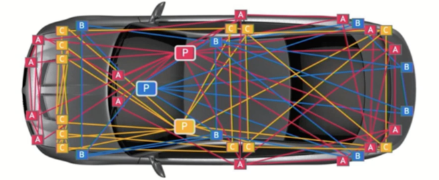
\includegraphics[width=\textwidth]{img/domain_architecture}
        \caption{\textit{Domain Architecture}}
        
        \begin{flushleft}
            \begin{enumerate}[nosep]
                \item central domain controller (\textbf{P}) or high performance computer
                \item ability to handle more complex functions
                \item cost optimization
                \item cable harness is rigid and expensive
            \end{enumerate}
        \end{flushleft}

    \end{minipage}
    \begin{minipage}[t]{0.45\textwidth}
        \centering
        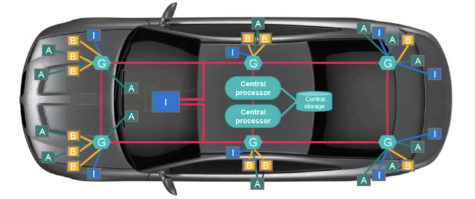
\includegraphics[width=\textwidth]{img/zonal_architecture}
        \caption{\textit{Zonal Architecture}}
        
        \begin{flushleft}
            \begin{enumerate}[nosep]
                \item local ethernet per zone (\textbf{G})
                \item ultra high-speed secured backbone between zone
                \item centralized software
                \item central computer storage
            \end{enumerate}
        \end{flushleft}
        
    \end{minipage}
\end{figure}
\chapter{Non Real-time scheduling algorithms}
Lo \textit{scheduling} è l'attività che permette di selezionare quale processo o \textit{thread} bisogna eseguire come successivo. In generale nei sistemi operativi, possiamo distinguere tre tipologie di \textit{scheduling}:
\begin{itemize}
    \item \textbf{\textit{long term scheduling}}: prima di creare il processo, viene deciso se attivarlo o meno. Viene implementato tramite un \textbf{test di ammissione}, se il processo passa questo controllo allora viene inserito nella \textit{ready queue}, se no viene interrotto finché non gli viene permesso di essere \textit{schedulato} [ se il \textit{load} del processore è troppo alto il nuovo task rischia di essere solo di ``intralcio'' ].
    \item \textbf{\textit{medium term scheduling}}: permette di decidere se un processo deve essere \textit{preemptato} o meno.
    \item \textbf{\textit{short term scheduling}}: decide quale processo deve essere eseguito come successivo. Possiamo distinguere:
    \begin{itemize}
        \item \textbf{\textit{selection function}}: decide quale processo viene selezionato dalla \textit{ready queue}, seguendo alcune regole.
        \item \textbf{\textit{decision mode}}: quando la decisione è stata presa si può comportare in maniera \textbf{\textit{preemptive}} oppure \textbf{\textit{non-preemptive}}.
    \end{itemize}
\end{itemize}
\textbf{\textit{Scheduling Criteria}}: come si possono valutare le performance di uno \textit{scheduler}:
\begin{itemize}
    \item \textbf{\textit{user-oriented}}: si va ad analizzare il \textit{response-time} del processo.
    \item \textbf{\textit{system-oriented}}: si va ad analizzare il \textit{throughput}, ovvero quanto lavoro il sistema può eseguire in un certo intervallo di tempo.
\end{itemize}
Per quanto le performance siano importanti in certe circostate ci possono interessare la \textbf{predicibitilà} (\textit{real-time system}) o la \textbf{\textit{fairness}}. \\
Tra i processi possiamo differenziare anche il tipo di risorsa che viene utilizzanta: \textbf{\textit{CPU-Bound}} e \textbf{\textit{I/O Bound}}, nel primo caso il processo è orientato a lavorare sul processore, mentre nel secondo caso i processi possono essere in attesa di un \textit{I/O device}. La stragrande maggioranza dei processi è un mix dei due. \\ \newline
Uno \textit{schedule} $\sigma$ si dice \textbf{fattibile} (\textbf{\textit{feasible}}) se tutti i \textit{tasks} sono capaci di completare entro un insieme di vincoli. \\
Un \textit{tasks set} $\mathcal{T}$ si dice \textbf{\textit{schedulable}} se esiste uno \textit{schedule} fattibile per esso. \\ \newline
\textbf{\textit{The General Scheduling Problem}}: dato un \textit{tasks set} $\mathcal{T}$ di $n$ \textit{tasks}, un set $\mathcal{P}$ di $m$ processori e un set $\mathcal{R}$ di $r$ risorse, trovare un assegnamento di $\mathcal{P}$ e $\mathcal{R}$ per $\mathcal{T}$ che produce uno \textit{schedule} fattibile. \\
È stato dimostrato nel 1975 da Garey e Johnson che il \textit{general scheduling problem} rientra nella categoria \textbf{\textit{NP hard}}. È però possibile, rilassando i vincoli e specificando certe condizioni, ricordurci ad un algoritmo \textit{polynomial time}. \\
Per il ora consideriamo:
\begin{itemize}
    \item processore singolo
    \item \textit{fully preemptive tasks}
    \item attivazione simultanea
    \item nessun vincolo di precedenza
    \item nessun vincolo sulle risorse
\end{itemize}

\begin{tabular}{ |p{7.25cm}|p{7.25cm}| }
    \hline
    \multicolumn{2}{|c|}{\textbf{Algorithm taxonomy}} \\
    \hline
    \textbf{\textit{preemptive}} & \textbf{\textit{non-preemptive}} \\
    \hline
    \textbf{\textit{off line}}: & \textbf{\textit{on line}}: \\
    tutte le decisioni sullo scheduling vengono prese prima dell'attivazione dei task, normalmente lo \textit{schedule} viene salvato in una tabella (\textbf{\textit{table-driven scheduling}}) & le decisioni di scheduling vengono prese \textit{runtime} sul set dei tasks attivi \\ \hline
    \textbf{\textit{static}}: & \textbf{\textit{dynamic}}: \\
    le decisioni di scheduling vengono prese basandosi su parametri fissati, staticamente assegnati al task prima dell'attivazione & le decisioni di scheduling vengono prese su parametri che possono variare nel tempo \\ \hline
    \textbf{\textit{best effort}}: & \textbf{\textit{optimal}}: \\
    trova sempre uno \textit{schedule} fattibile, se \textbf{esiste} & fa del suo meglio per trovare uno \textit{schedule} fattibile, se esiste, ma non lo garantisce. \\ \hline
\end{tabular}
\\ \newline
Le \textit{policies} classiche di \textbf{\textit{scheduling}}, che però non sono adatte per sistemi \textit{real-time}, sono:
\begin{enumerate}

    \item \textbf{\textit{First Come First Served} (FCFS)}: assegna l'utilizzo della CPU al task basandosi sull'ordine di arrivo, non è \textit{preemptive}, è dinamico, online e \textit{best effort}. \\
    $\rightarrow$ molto \textbf{impredicibile}: il \textit{response time} è fortemente dipendente dall'ordine di arrivo dei task.

    \item \textbf{\textit{Shorter Job First} (SJF)}: seleziona il task che ha il minor \textit{computational time}, può essere sia \textit{preemptive} che \textit{non-preemptive}, è statico (il parametro $C_i$ è fissato da configurazione), può essere usato sia \textit{online} che \textit{off-line} e permette di minimizzare la \textit{response time} \textbf{media}. \\
    \textcolor{green}{\textbf{Dimostrazione dell'ottimalità di SJF}}: consideriamo uno scheduler $\sigma \neq \text{SJF}$ e un'altro scheduler $\sigma'$ che è uguale a SJF fino all'istante $f_s$
    \begin{figure}[h]
        \centering
        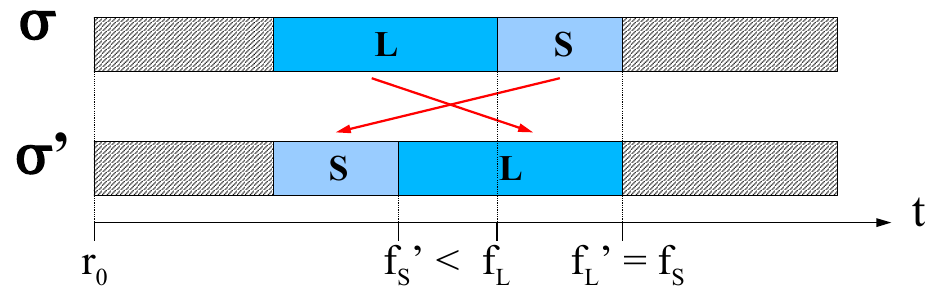
\includegraphics[width=0.4\textwidth]{img/sjf_opt}    
    \end{figure}
    \\ 
    Presi due task $L$ e $S$ che hanno \textit{request time} $r_i \; i \in \{L, S\}$ e \textit{finish time} $f_i \; i \in \{L, S\}$. Lo \textit{schedule} $\sigma$ schedula il task $L$ prima (non conforme con SJF), mentre $\sigma'$ schedula il task $S$ come primo (conforme a SJF). Possiamo dire che $f'_L = f_S$ in quanto la somma del tempo dei due task non cambia, ma cambia solo l'ordine di schedulazione. È intuitivo che il \textit{finish time} del primo task è però sbilanciato verso lo scheduler $\sigma'$ infatti avremo $f'_S < f_L$. \\
    Avremo perciò $f'_S + f'_L \leq f_S + f_L$ 
    \begin{center}
        $\rightarrow \qquad \bar{R}(\sigma') = \frac{1}{n} \cdot \sum_{i = 1}^{n}{(f'_i - r_i)} \leq \frac{1}{n} \cdot \sum_{i = 1}^{n}{(f_i - r_i)} = \bar{R}(\sigma)$
    \end{center}
    Lo scheduler $\sigma'$ è equivalente a SJF solo fino all'istante $f'_L = f_S$, bisogna andare quindi ad iterare su ogni scheduler $\sigma \in \{\sigma', \sigma'', ..., \sigma^*\}$, andando a riproporre l'analisi appena condotta avremo che: $\bar{R}(\sigma) \geq \bar{R}(\sigma') \geq \bar{R}{\sigma''} \geq \cdots \geq \bar{R}(\sigma^*)$ \\
    $\rightarrow$ $\sigma^* = \sigma_{sjf}$ e quindi avremo che $\bar{R}(\sigma_{SJF})$ è la \textbf{minima \textit{response time} media} ottenibile da ogni \textbf{algoritmo}. \\
    \textbf{SJF non è un algoritmo fattibile per il \textit{Real-Time}}.

    \item \textbf{\textit{Priority Scheduling}}
\end{enumerate}
\chapter{Real-time scheduling algorithms}


% PAGINA VUOTA
%\clearpage\null\thispagestyle{empty}\clearpage
%\appendix
%\appendixpage
%\addappheadtotoc

%\clearpage\null\thispagestyle{empty}\clearpage


%\listoffigures


\begin{flushleft}
\bibliographystyle{plain}
\bibliography{sections/references} 
\end{flushleft}

\end{document}
